\documentclass[12pt]{article}

% TEMPLATE DEFAULT PACKAGES
\usepackage{amssymb,amsmath,amsfonts,eurosym,geometry,ulem,graphicx,color,setspace,sectsty,comment,natbib,pdflscape,array,adjustbox}

% ADDED PACKAGES FOR THIS MANUSCRIPT
\usepackage{palatino,newtxmath,multirow,titlesec,threeparttable,tabu,booktabs,titlesec,threeparttable,mathtools,bm,bbm,subcaption,pdflscape,tcolorbox,mathrsfs,tikz,graphicx}
% endfloat,

\usepackage{afterpage}
\usepackage[hyphens]{url}
\usepackage[margin=1cm]{caption}

\usepackage[draft]{hyperref}
\newcommand{\tim}{$\,\times\,$}
% FIGURES & TABLES CAPTION STYLING
\captionsetup[figure]{labelfont={bf},name={Figure},labelsep=period}
\captionsetup[table]{labelfont={bf},name={Table},labelsep=period}

% SECTION TITLE SETTINGS
\titlelabel{\thetitle.\enskip}
\titleformat*{\section}{\large\bfseries}
\titleformat*{\subsection}{\normalsize\bfseries}

% COLUMN TYPES
\newcolumntype{L}[1]{>{\raggedright\let\newline\\\arraybackslash\hspace{0pt}}m{#1}}
\newcolumntype{C}{>{\centering\arraybackslash}p{5.2em}}
\newcolumntype{D}{>{\centering\arraybackslash}p{5em}}
\newcolumntype{R}[1]{>{\raggedleft\let\newline\\\arraybackslash\hspace{0pt}}m{#1}}


% MARGINS AND SPACING
\normalem
\geometry{left=1.1in,right=1.1in,top=1.0in,bottom=1.0in}
\setlength{\parskip}{2.5pt}

% SPECIAL CELL 
\newcommand{\specialcell}[2][c]{%
	\begin{tabular}[#1]{@{}l@{}}#2\end{tabular}}

% NO INDENT ON FOOTNOTES
\usepackage[hang,flushmargin]{footmisc}

\begin{document}








\vspace{0mm}
\begin{table}[h!]
\centering
\caption{Housing Project Areas Description}\label{table:projectdescriptives}
\vspace{0mm}
\begin{tabular}{l*{1}{cccccc}}
\toprule
  & \multicolumn{2}{c}{\textbf{All}}& \multicolumn{2}{c}{\textbf{Greenfield}}  & \multicolumn{2}{c}{\textbf{In-Situ}}   \\
  &Const. & Unconst. &Const. & Unconst.   & Const. & Unconst. \\
\midrule
 Number of Projects  & 172  & 145  & 43  & 20  & 27  & 29  \\ 
 Area (km2)  & 1.17  & 1.16  & 1.72  & 2.42  & 1.50  & 0.88  \\ 
 Median Construction Yr.  & 2006  & 2006  & 2006  & 2005  & 2004  & 2006  \\ 
 Delivered Houses  & 374  & 11  & 568  & 24  & 702  & 20  \\ 
 House Price in 1 km (R$^\dagger$)  & 188,441  & 218,635  & 194,214  & 186,841  & 179,596  & 208,570  \\ 
 Distance to CBD$^\ddagger$ (km)  & 32.5  & 27.7  & 40.5  & 39.9  & 32.6  & 30.6  \\ 

\bottomrule
\multicolumn{7}{l}{\scriptsize Const. refers to constructed projects and unconst. refers to unconstructed projects.}\\[-.5em]
\multicolumn{7}{l}{\scriptsize $^*$Calculated from {\it expected} completion dates using Gauteng National Treasury budget reports.}\\[-.5em]
\multicolumn{7}{l}{\scriptsize $^\dagger$ The USD averaged to about 7.70 Rands during the 2001-2011 period.}\\[-.5em]
\multicolumn{7}{l}{\scriptsize $^\ddagger$Measured as the average minimum distance with respect to Johannesburg and Pretoria CBDs. } \\[-.5em]
%\multicolumn{7}{l}{\scriptsize City includes projects whose centroids are within 30.4 km of their nearest CBD.} \\[-.5em]
%\multicolumn{7}{l}{\scriptsize Suburb includes projects whose centroids are further than 30.4 km from their nearest CBD.}
\end{tabular}
\end{table} 



\begin{table}
\begin{tabular}{lDDDDD}
\toprule
 & \small (1) & \small (2)  & \small (3) & \small (4) & \small (5) \\
 & Total & Formal  & Informal & Informal Bkyd. & Informal Non-Bkyd. \\ \midrule
inside project      &     649.922\textsuperscript{a}&     578.443\textsuperscript{a}&      71.480                   &     504.849\textsuperscript{a}&    -433.370\textsuperscript{a}\\
                    &   (142.583)                   &    (74.803)                   &   (109.399)                   &   (103.801)                   &    (87.272)                   \\[0.55em]
0-300m outside project &      -4.615                   &      34.561                   &     -39.176                   &       6.232                   &     -45.408                   \\
                    &    (43.547)                   &    (24.463)                   &    (35.468)                   &    (31.659)                   &    (28.679)                   \\[0.5em]
300-600m outside project &     -93.284\textsuperscript{b}&      -4.618                   &     -88.666\textsuperscript{a}&     -65.122\textsuperscript{b}&     -23.544                   \\
                    &    (37.619)                   &    (16.266)                   &    (33.159)                   &    (28.282)                   &    (16.891)                   \\[0.5em]
Mean Outcome 2001   &      379.90                   &      203.91                   &      175.98                   &       66.26                   &      109.72                   \\
Mean Outcome 2011   &      584.70                   &      281.66                   &      303.04                   &      192.77                   &      110.27                   \\
R$^2$               &       0.095                   &       0.064                   &       0.079                   &       0.059                   &       0.052                   \\
\# projects         &         308                   &         308                   &         308                   &         308                   &         308                   \\
N project areas     &     266,572                   &     266,572                   &     266,572                   &     266,572                   &     266,572                   \\
N spillover areas   &     501,926                   &     501,926                   &     501,926                   &     501,926                   &     501,926                   \\
N                   &   2,721,910                   &   2,721,910                   &   2,721,910                   &   2,721,910                   &   2,721,910                   \\

\bottomrule
\end{tabular}
\end{table}


\begin{table}
 \resizebox{\linewidth}{!}{
\begin{tabular}{lDDDDD}
\toprule
 & \small (1) & \small (2)  & \small (3) & \small (4) & \small (5) \\
 & Total & Formal  & Informal & Informal Bkyd. & Informal Non-Bkyd. \\ \midrule
\textbf{Greenfield} \\   inside project      &     217.909                   &     222.695\textsuperscript{c}&      -4.785                   &      79.224                   &     -84.009                   \\
                    &   (213.941)                   &   (119.653)                   &   (111.448)                   &   (124.833)                   &    (62.730)                   \\[0.01em]
0-300m outside project &     -44.056                   &       9.956                   &     -54.012                   &     -43.341                   &     -10.671                   \\
                    &    (78.251)                   &    (30.002)                   &    (59.637)                   &    (57.969)                   &    (35.938)                   \\[0.01em]
300-600m outside project&     -81.483\textsuperscript{c}&     -20.464                   &     -61.019\textsuperscript{b}&     -45.399\textsuperscript{c}&     -15.620                   \\
                    &    (46.495)                   &    (26.880)                   &    (30.145)                   &    (23.782)                   &    (19.042)                   \\[0.8em] 
\textbf{In-Situ Upgrading} \\   inside project      &     695.310\textsuperscript{c}&     921.289\textsuperscript{a}&    -225.979                   &     700.269\textsuperscript{b}&    -926.248\textsuperscript{a}\\
                    &   (386.705)                   &   (166.130)                   &   (283.422)                   &   (270.238)                   &   (235.351)                   \\[0.01em]
0-300m outside project &     178.887                   &     200.068\textsuperscript{c}&     -21.180                   &      70.923                   &     -92.103                   \\
                    &   (193.903)                   &   (120.530)                   &   (117.670)                   &   (141.136)                   &    (96.654)                   \\[0.01em]
300-600m outside project &     111.841                   &     176.224\textsuperscript{c}&     -64.383                   &     -32.190                   &     -32.193                   \\
                    &   (141.919)                   &    (94.980)                   &    (85.051)                   &    (97.611)                   &    (70.292)                   \\[0.8em]
\textbf{Other} \\   inside project      &     778.199\textsuperscript{a}&     659.434\textsuperscript{a}&     118.765                   &     615.013\textsuperscript{a}&    -496.249\textsuperscript{a}\\
                    &   (190.566)                   &    (85.015)                   &   (166.248)                   &   (133.791)                   &    (93.505)                   \\[0.01em]
0-300m outside project &    -171.670\textsuperscript{b}&     -24.877                   &    -146.793\textsuperscript{b}&     -37.050                   &    -109.743\textsuperscript{a}\\
                    &    (84.637)                   &    (32.861)                   &    (65.637)                   &    (53.607)                   &    (41.974)                   \\[0.01em]
300-600m outside project &    -220.388\textsuperscript{a}&     -77.165\textsuperscript{a}&    -143.223\textsuperscript{a}&     -82.017\textsuperscript{c}&     -61.206\textsuperscript{b}\\
                    &    (69.087)                   &    (27.133)                   &    (54.004)                   &    (47.646)                   &    (25.964)                   \\[0.8em]
Mean Outcome 2001   &      379.90                   &      203.91                   &      175.98                   &       66.26                   &      109.72                   \\
Mean Outcome 2011   &      584.70                   &      281.66                   &      303.04                   &      192.77                   &      110.27                   \\
R$^2$               &       0.125                   &       0.079                   &       0.106                   &       0.081                   &       0.069                   \\
\# projects         &         308                   &         308                   &         308                   &         308                   &         308                   \\
N project areas     &     266,572                   &     266,572                   &     266,572                   &     266,572                   &     266,572                   \\
N spillover areas   &     501,926                   &     501,926                   &     501,926                   &     501,926                   &     501,926                   \\
N                   &   2,721,910                   &   2,721,910                   &   2,721,910                   &   2,721,910                   &   2,721,910                   \\

\bottomrule
\end{tabular}
}
\end{table}


\afterpage{%
  \clearpage% 
\begin{landscape}
{\footnotesize
\begin{table}[]
\small
\centering
\caption{Census Household-level Estimates}\label{table:censusestimates}
\vspace{-2mm}
\begin{tabular}{lDDDDDDDD}
\toprule
 & \small (1) & \small (2)  & \small (3) & \small (4) & \small (5)  & \small (6)  & \small (7) & (8)\\
 & \small Flush Toilet & \small Water Indoors  & \small Electricity Cooking & \small Electricity Heating & \small Electricity Lighting  & \small Number of Rooms  & \small Household Size & Population Density\\ \midrule 
inside $\times$ constr $\times$ post&       0.101                   &      -0.022                   &       0.165\textsuperscript{b}&       0.126\textsuperscript{c}&       0.045                   &      -0.282\textsuperscript{c}&       0.255\textsuperscript{b}&   -1323.017                   \\
                    &     (0.076)                   &     (0.040)                   &     (0.074)                   &     (0.068)                   &     (0.079)                   &     (0.150)                   &     (0.099)                   &  (1652.834)                   \\[0.55em]
0-200m out $\times$ constr $\times$ post&      -0.029                   &      -0.096\textsuperscript{b}&      -0.036                   &      -0.005                   &      -0.067                   &      -0.230                   &       0.160\textsuperscript{b}&     473.519                   \\
                    &     (0.049)                   &     (0.046)                   &     (0.044)                   &     (0.049)                   &     (0.044)                   &     (0.152)                   &     (0.066)                   &  (1108.833)                   \\[0.5em]
200-400m out $\times$ constr $\times$ post&      -0.015                   &      -0.158\textsuperscript{a}&      -0.030                   &      -0.012                   &      -0.054\textsuperscript{c}&      -0.245\textsuperscript{b}&       0.206\textsuperscript{a}&    -379.912                   \\
                    &     (0.035)                   &     (0.035)                   &     (0.035)                   &     (0.038)                   &     (0.030)                   &     (0.114)                   &     (0.051)                   &   (770.742)                   \\[0.5em]
Mean Outcome 2001   &        0.82                   &        0.42                   &        0.71                   &        0.68                   &        0.80                   &        3.47                   &        3.40                   &    8,381.79                   \\
Mean Outcome 2011   &        0.85                   &        0.60                   &        0.82                   &        0.74                   &        0.85                   &        3.84                   &        3.11                   &    8,792.50                   \\
R$^2$               &       0.322                   &       0.375                   &       0.384                   &       0.370                   &       0.344                   &       0.383                   &       0.407                   &       0.292                   \\
\# projects         &         314                   &         314                   &         314                   &         314                   &         314                   &         314                   &         314                   &         314                   \\
N project areas     &       3,659                   &       3,659                   &       3,659                   &       3,659                   &       3,659                   &       3,653                   &       3,659                   &       3,659                   \\
N spillover areas   &       2,849                   &       2,849                   &       2,849                   &       2,849                   &       2,849                   &       2,844                   &       2,847                   &       2,849                   \\
N                   &      17,499                   &      17,499                   &      17,499                   &      17,499                   &      17,499                   &      17,463                   &      17,488                   &      17,501                   \\

\bottomrule
\multicolumn{9}{l}{\footnotesize All regressions include project Fixed-Effects. Standard errors clustered at the project level in parenthesis. \textsuperscript{c} p$<$0.10,\textsuperscript{b} p$<$0.05,\textsuperscript{a} p$<$0.01 }
\end{tabular}
\end{table}
}
\end{landscape}
}

\afterpage{%
  \clearpage% 
\begin{landscape}
{\footnotesize
\begin{table}[]
\small
\centering
\caption{Census Household-level Estimates By Type of Project}\label{table:censusestimates}
\vspace{-2mm}
\begin{tabular}{lDDDDDDDD}
\toprule
 & \small (1) & \small (2)  & \small (3) & \small (4) & \small (5)  & \small (6)  & \small (7) & (8)\\
 & \small Flush Toilet & \small Water Indoors  & \small Electricity Cooking & \small Electricity Heating & \small Electricity Lighting  & \small Number of Rooms  & \small Household Size & Population Density\\ \midrule 
Green inside $\times$ constr $\times$ post &      -0.125                   &      -0.111                   &      -0.116                   &      -0.148                   &      -0.181                   &      -0.549\textsuperscript{b}&       0.311\textsuperscript{a}&    4532.190\textsuperscript{c}\\
                    &     (0.190)                   &     (0.109)                   &     (0.127)                   &     (0.125)                   &     (0.152)                   &     (0.244)                   &     (0.114)                   &  (2606.250)                   \\[0.01em]
Green 0-200m out $\times$ constr $\times$ post&       0.020                   &      -0.013                   &      -0.031                   &       0.040                   &      -0.005                   &       0.414\textsuperscript{c}&       0.531\textsuperscript{a}&   -1454.402                   \\
                    &     (0.057)                   &     (0.112)                   &     (0.079)                   &     (0.093)                   &     (0.044)                   &     (0.244)                   &     (0.119)                   &  (1003.651)                   \\[0.01em]
Green 200-400m out $\times$ constr $\times$ post&      -0.071                   &      -0.215\textsuperscript{a}&      -0.057                   &      -0.017                   &       0.003                   &      -0.378                   &       0.270\textsuperscript{b}&    -106.627                   \\
                    &     (0.065)                   &     (0.069)                   &     (0.078)                   &     (0.095)                   &     (0.057)                   &     (0.323)                   &     (0.121)                   &   (817.142)                   \\[0.5em]
In-Situ inside $\times$ constr $\times$ post &       0.266\textsuperscript{c}&      -0.064                   &       0.074                   &       0.077                   &       0.015                   &      -0.061                   &       0.403\textsuperscript{b}&   -4469.706                   \\
                    &     (0.144)                   &     (0.085)                   &     (0.107)                   &     (0.096)                   &     (0.103)                   &     (0.219)                   &     (0.180)                   &  (3143.592)                   \\[0.01em]
In-Situ 0-200m out $\times$ constr $\times$ post&      -0.090                   &      -0.175\textsuperscript{c}&      -0.121                   &      -0.111                   &      -0.101                   &      -0.489\textsuperscript{b}&       0.208\textsuperscript{c}&   -2024.208\textsuperscript{c}\\
                    &     (0.096)                   &     (0.092)                   &     (0.077)                   &     (0.090)                   &     (0.081)                   &     (0.226)                   &     (0.123)                   &  (1206.841)                   \\[0.01em]
In-Situ 200-400m out $\times$ constr $\times$ post&      -0.040                   &      -0.230\textsuperscript{a}&      -0.112\textsuperscript{c}&      -0.115                   &      -0.094\textsuperscript{c}&      -0.503\textsuperscript{a}&       0.266\textsuperscript{a}&    -970.981                   \\
                    &     (0.071)                   &     (0.069)                   &     (0.065)                   &     (0.079)                   &     (0.050)                   &     (0.183)                   &     (0.074)                   &  (1078.809)                   \\[0.5em]
Other inside $\times$ constr $\times$ post &      -0.024                   &      -0.028                   &       0.140                   &       0.109                   &       0.038                   &      -0.365\textsuperscript{c}&       0.250\textsuperscript{b}&   -1083.328                   \\
                    &     (0.093)                   &     (0.049)                   &     (0.108)                   &     (0.102)                   &     (0.119)                   &     (0.208)                   &     (0.127)                   &   (994.953)                   \\[0.01em]
Other 0-200m out $\times$ constr $\times$ post&      -0.024                   &      -0.112\textsuperscript{b}&      -0.063                   &      -0.007                   &      -0.077                   &      -0.156                   &       0.204\textsuperscript{b}&     742.657                   \\
                    &     (0.052)                   &     (0.048)                   &     (0.053)                   &     (0.055)                   &     (0.051)                   &     (0.171)                   &     (0.083)                   &  (1578.655)                   \\[0.01em]
Other 200-400m out $\times$ constr $\times$ post&      -0.004                   &      -0.114\textsuperscript{a}&      -0.037                   &       0.000                   &      -0.045                   &      -0.036                   &       0.277\textsuperscript{a}&   -1838.043\textsuperscript{b}\\
                    &     (0.040)                   &     (0.043)                   &     (0.041)                   &     (0.043)                   &     (0.039)                   &     (0.133)                   &     (0.072)                   &   (933.431)                   \\[0.5em]
Mean Outcome 2001   &        0.78                   &        0.34                   &        0.63                   &        0.60                   &        0.75                   &        3.25                   &        3.51                   &    8,544.01                   \\
Mean Outcome 2011   &        0.83                   &        0.52                   &        0.80                   &        0.70                   &        0.81                   &        3.51                   &        3.17                   &    9,932.98                   \\
R$^2$               &       0.402                   &       0.391                   &       0.463                   &       0.434                   &       0.425                   &       0.436                   &       0.482                   &       0.397                   \\
\# projects         &         313                   &         313                   &         313                   &         313                   &         313                   &         313                   &         313                   &         313                   \\
N project areas     &       3,655                   &       3,655                   &       3,655                   &       3,655                   &       3,655                   &       3,649                   &       3,655                   &       3,655                   \\
N spillover areas   &       2,849                   &       2,849                   &       2,849                   &       2,849                   &       2,849                   &       2,844                   &       2,847                   &       2,849                   \\
N                   &      11,470                   &      11,470                   &      11,470                   &      11,470                   &      11,470                   &      11,448                   &      11,468                   &      11,471                   \\

\bottomrule
\multicolumn{9}{l}{\footnotesize All regressions include project Fixed-Effects. Standard errors clustered at the project level in parenthesis. \textsuperscript{c} p$<$0.10,\textsuperscript{b} p$<$0.05,\textsuperscript{a} p$<$0.01 }
\end{tabular}
\end{table}
}
\end{landscape}
}







\begin{figure*}
        %\vspace{2mm}
        \begin{subfigure}[b]{0.495\textwidth}
            \centering
        \caption{Formal}
            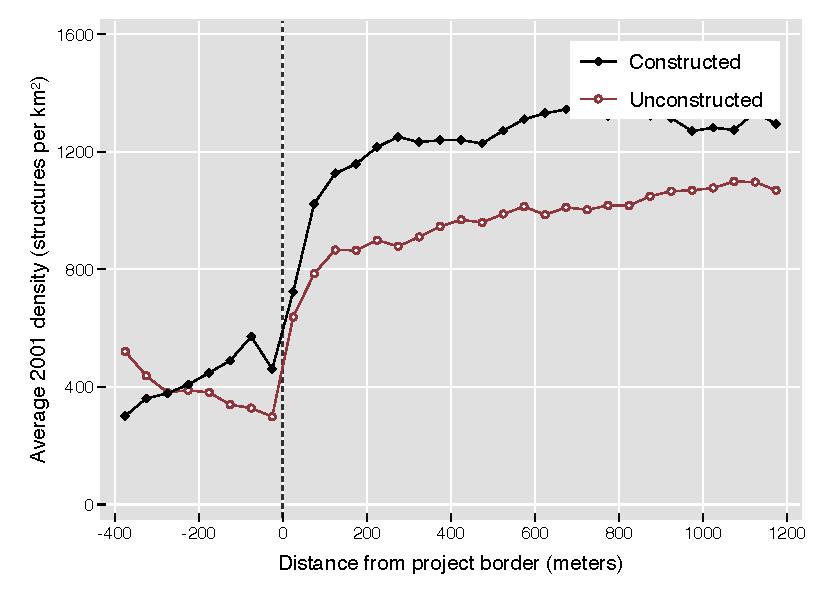
\includegraphics[width=\textwidth,trim={0.3cm .3cm 0.1cm 0cm}, clip=true]{figures/bblu_for_pre_means_4}
        \end{subfigure}
        \hfill
        \begin{subfigure}[b]{0.495\textwidth}  
            \centering 
        \caption{ Informal}
            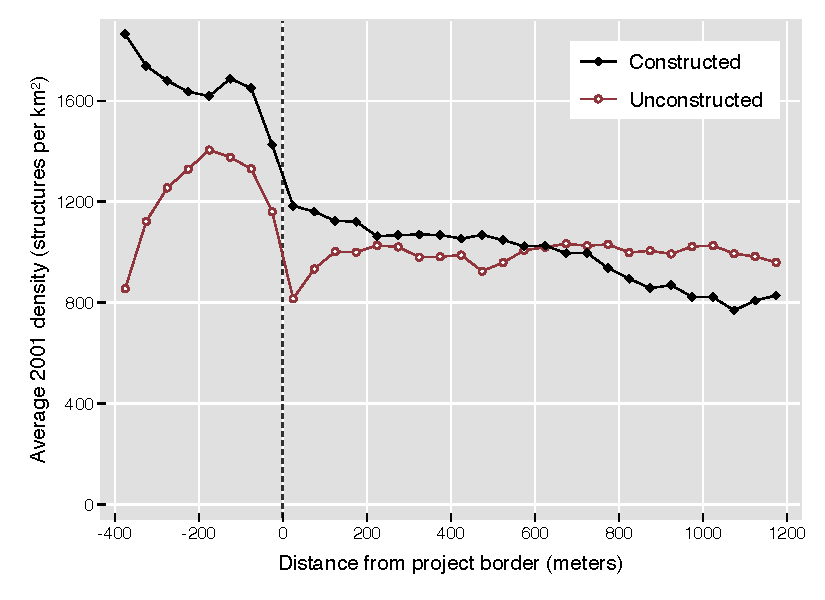
\includegraphics[width=\textwidth,trim={0.3cm .3cm 0.1cm 0cm}, clip=true]{figures/bblu_inf_pre_means_4.pdf}
        \end{subfigure}
        %\vspace{2mm}
        \begin{subfigure}[b]{0.495\textwidth}
            \centering
        \caption{Formal}
            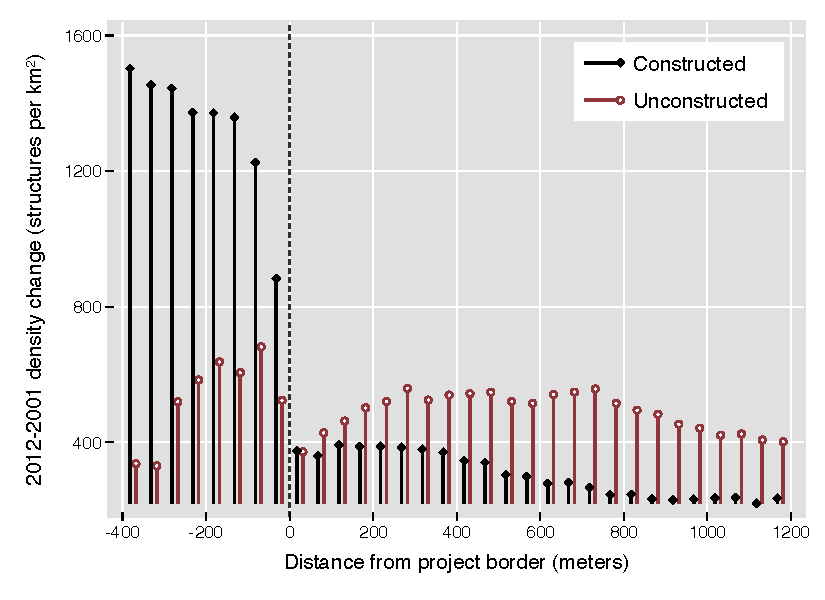
\includegraphics[width=\textwidth,trim={0.3cm .3cm 0.1cm 0cm}, clip=true]{figures/bblu_for_rawchanges_4}
        \end{subfigure}
        \hfill
        \begin{subfigure}[b]{0.495\textwidth}  
            \centering 
        \caption{Informal}
            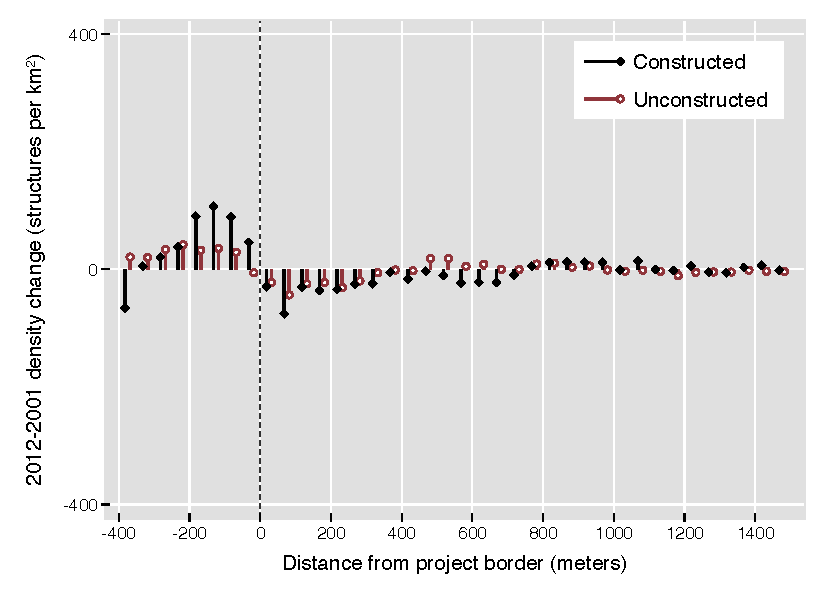
\includegraphics[width=\textwidth,trim={0.3cm .3cm 0.1cm 0cm}, clip=true]{figures/bblu_inf_rawchanges_4.pdf}
        \end{subfigure}
\end{figure*}



\begin{figure*}
        %\vspace{2mm}
        \begin{subfigure}[b]{0.495\textwidth}
            \centering
        \caption{Greenfield : Formal}
            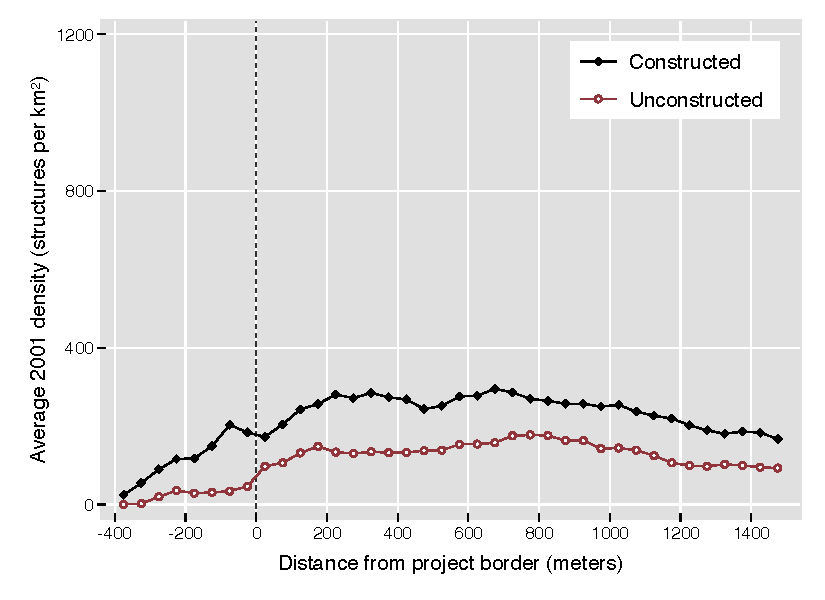
\includegraphics[width=\textwidth,trim={0.3cm .3cm 0.1cm 0cm}, clip=true]{figures/bblu_for_pre_means_4_1}
        \end{subfigure}
        \hfill
        \begin{subfigure}[b]{0.495\textwidth}  
            \centering 
        \caption{Greenfield : Informal}
            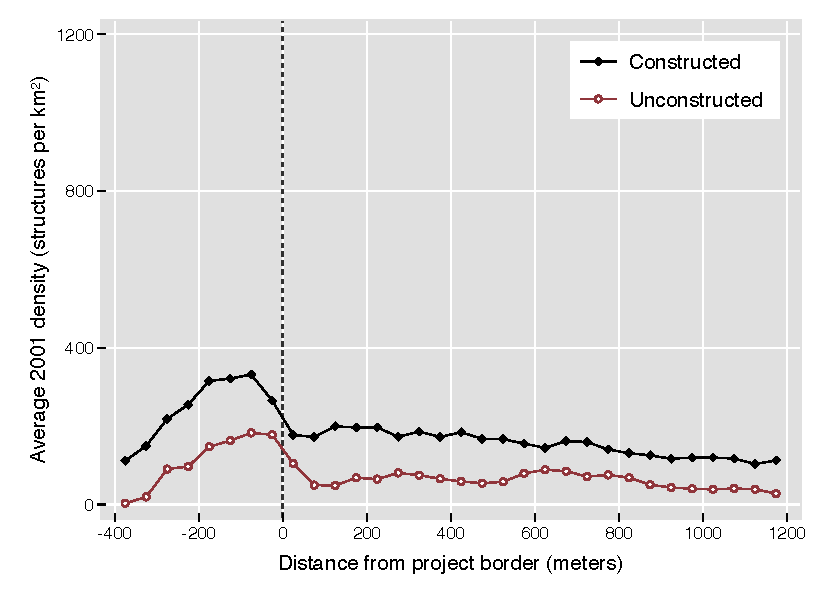
\includegraphics[width=\textwidth,trim={0.3cm .3cm 0.1cm 0cm}, clip=true]{figures/bblu_inf_pre_means_4_1.pdf}
        \end{subfigure}
        %\vspace{-6mm}
        %\vspace{2mm}
        \begin{subfigure}[b]{0.495\textwidth}
            \centering
        \caption{In-Situ Upgrading : Formal}
            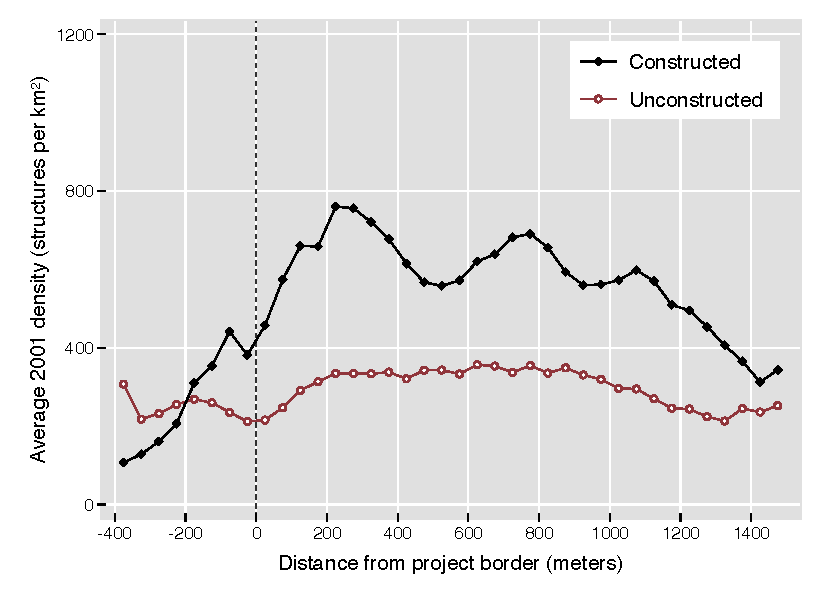
\includegraphics[width=\textwidth,trim={0.3cm .3cm 0.1cm 0cm}, clip=true]{figures/bblu_for_pre_means_4_2.pdf}
        \end{subfigure}
        \hfill
        %\vspace{2mm}
        \begin{subfigure}[b]{0.495\textwidth}
            \centering
        \caption{In-Situ Upgrading : Informal}
                %        Mixed Dev
            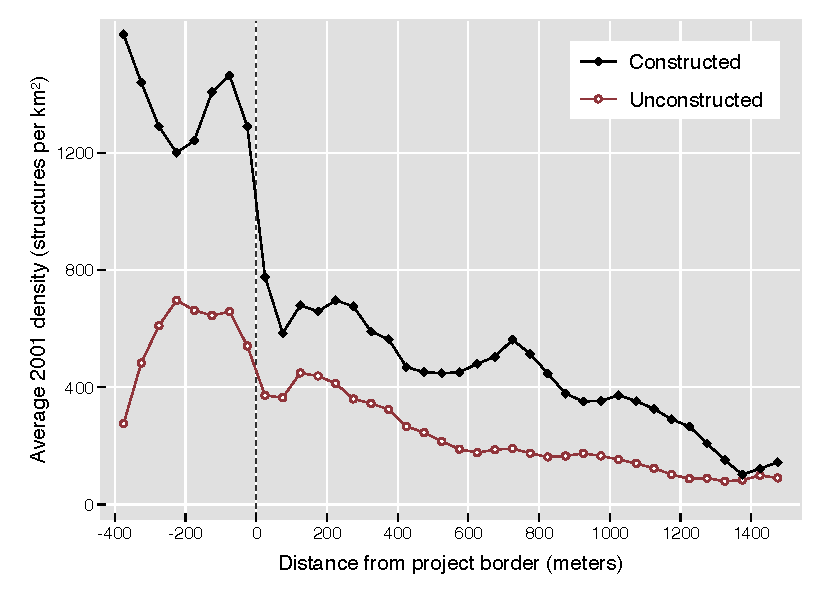
\includegraphics[width=\textwidth,trim={0.3cm .3cm 0.1cm 0cm}, clip=true]{figures/bblu_inf_pre_means_4_2.pdf}
        \end{subfigure}
                %\vspace{2mm}
        %\vspace{-6mm}
        \begin{subfigure}[b]{0.495\textwidth}  
            \centering 
            \caption{Other : Formal}
                %        Essential
            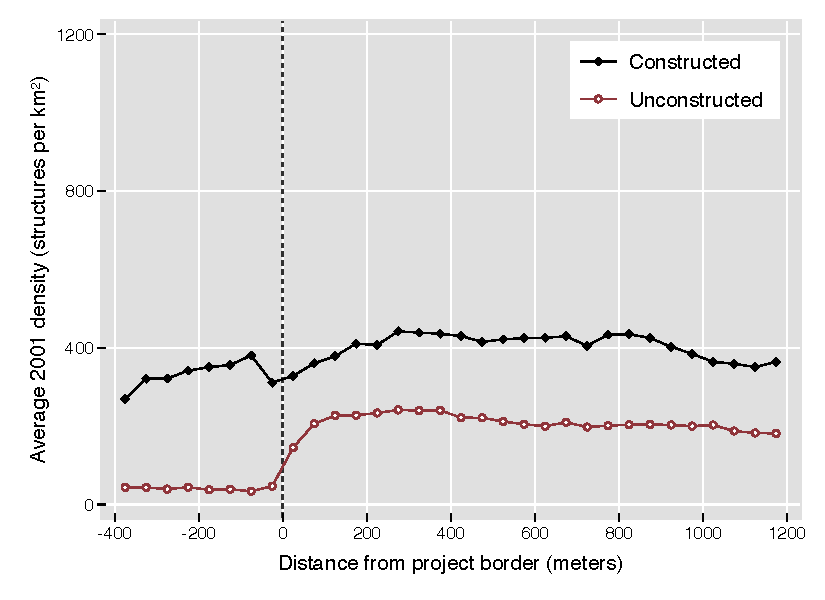
\includegraphics[width=\textwidth,trim={0.3cm .3cm 0.1cm 0cm}, clip=true]{figures/bblu_for_pre_means_4_3.pdf}
        \end{subfigure}
        \hfill
        %\vspace{2mm}
        \begin{subfigure}[b]{0.495\textwidth}
            \centering
            \caption{Other : Informal}
                  %      GDOH
            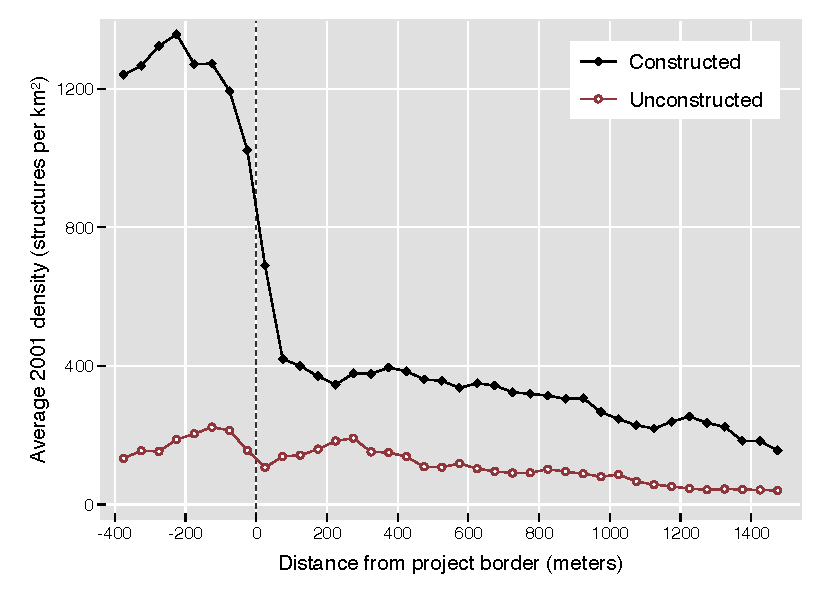
\includegraphics[width=\textwidth,trim={0.3cm .3cm 0.1cm 0cm}, clip=true]{figures/bblu_inf_pre_means_4_3.pdf}
        \end{subfigure}
        % \hfill
        % \begin{subfigure}[b]{0.495\textwidth}  
        %     \centering 
        %            %     Other
        %     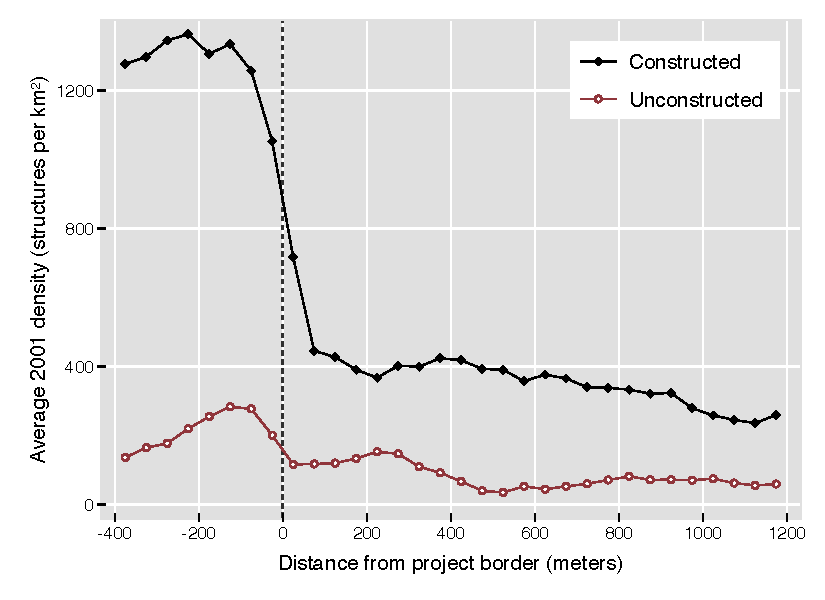
\includegraphics[width=\textwidth,trim={0.3cm .3cm 0.1cm 0cm}, clip=true]{figures/bblu_inf_pre_means_4_4.pdf}
        % \end{subfigure}
        % \vspace{-6mm}
    \end{figure*} 




\begin{figure*}
        %\vspace{2mm}
        \begin{subfigure}[b]{0.495\textwidth}
            \centering
        \caption{Greenfield : Formal}
            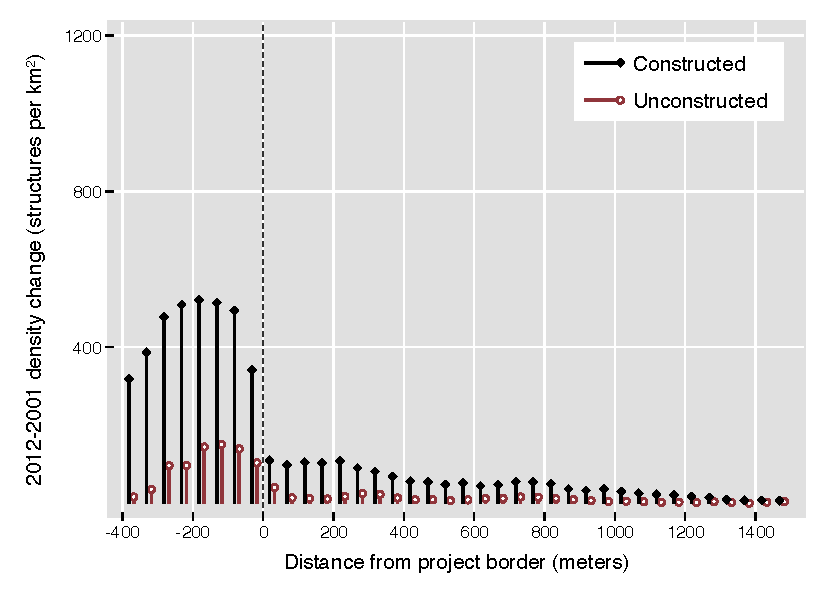
\includegraphics[width=\textwidth,trim={0.3cm .3cm 0.1cm 0cm}, clip=true]{figures/bblu_for_rawchanges_4_1}
        \end{subfigure}
        \hfill
        \begin{subfigure}[b]{0.495\textwidth}  
            \centering 
        \caption{Greenfield : Informal}
            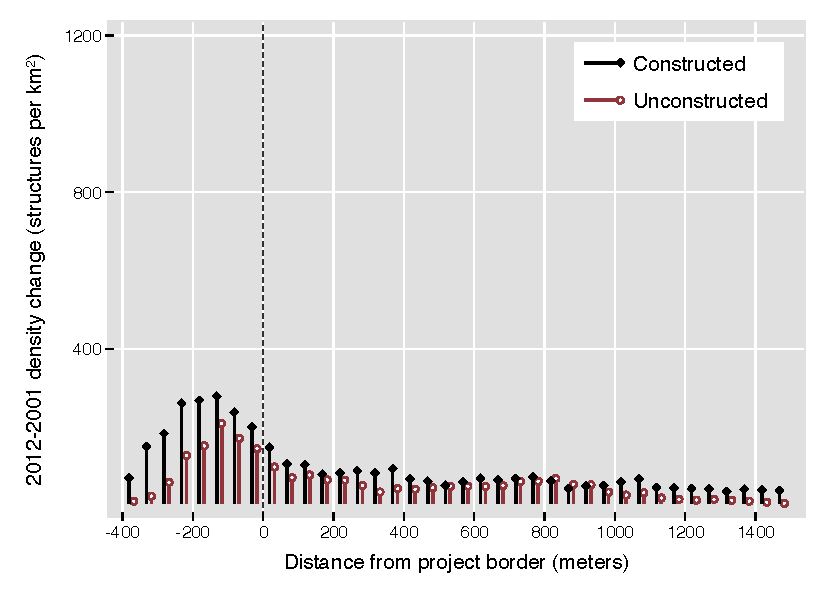
\includegraphics[width=\textwidth,trim={0.3cm .3cm 0.1cm 0cm}, clip=true]{figures/bblu_inf_rawchanges_4_1.pdf}
        \end{subfigure}
        %\vspace{-6mm}
        %\vspace{2mm}
        \begin{subfigure}[b]{0.495\textwidth}
            \centering
        \caption{In-Situ Upgrading : Formal}
            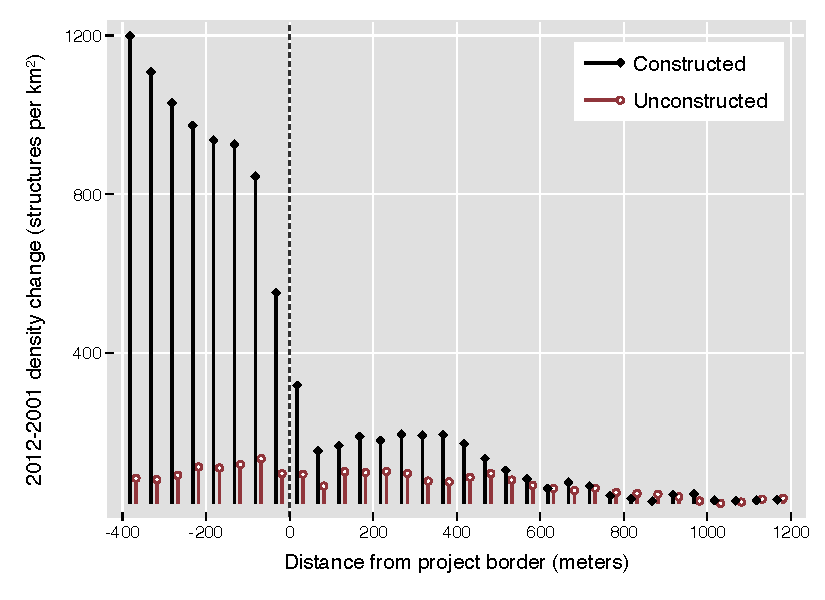
\includegraphics[width=\textwidth,trim={0.3cm .3cm 0.1cm 0cm}, clip=true]{figures/bblu_for_rawchanges_4_2.pdf}
        \end{subfigure}
        \hfill
        %\vspace{2mm}
        \begin{subfigure}[b]{0.495\textwidth}
            \centering
        \caption{In-Situ Upgrading : Informal}
                %        Mixed Dev
            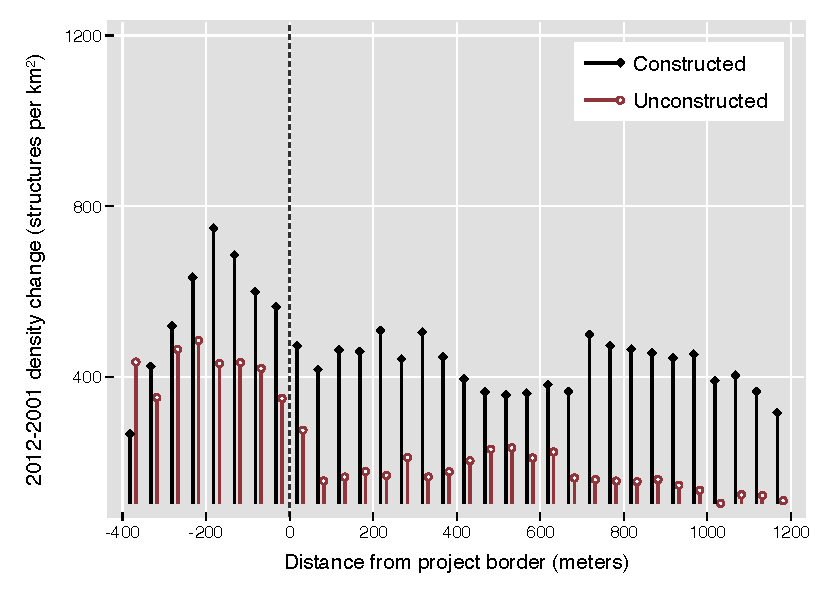
\includegraphics[width=\textwidth,trim={0.3cm .3cm 0.1cm 0cm}, clip=true]{figures/bblu_inf_rawchanges_4_2.pdf}
        \end{subfigure}
                %\vspace{2mm}
        %\vspace{-6mm}
        \begin{subfigure}[b]{0.495\textwidth}  
            \centering 
            \caption{Other : Formal}
                %        Essential
            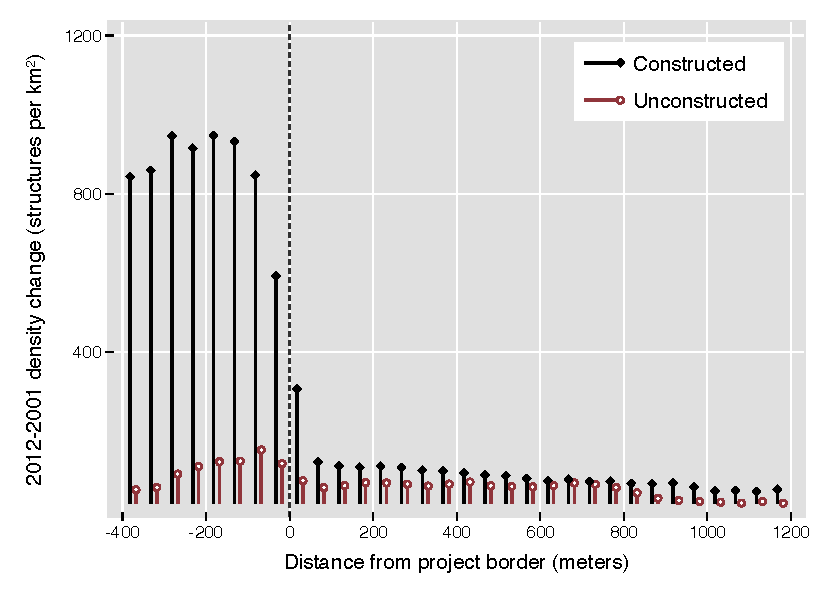
\includegraphics[width=\textwidth,trim={0.3cm .3cm 0.1cm 0cm}, clip=true]{figures/bblu_for_rawchanges_4_3.pdf}
        \end{subfigure}
        \hfill
        %\vspace{2mm}
        \begin{subfigure}[b]{0.495\textwidth}
            \centering
            \caption{Other : Informal}
                  %      GDOH
            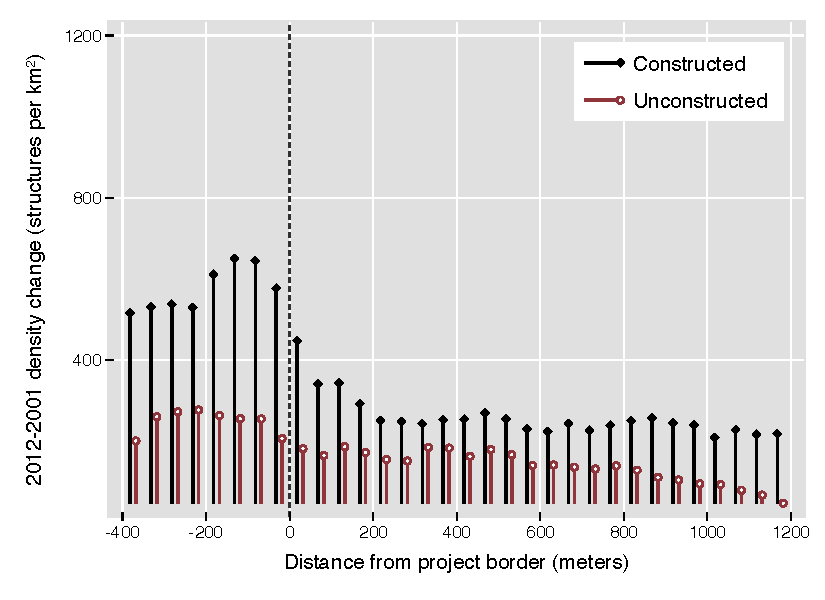
\includegraphics[width=\textwidth,trim={0.3cm .3cm 0.1cm 0cm}, clip=true]{figures/bblu_inf_rawchanges_4_3.pdf}
        \end{subfigure}
        % \hfill
        % \begin{subfigure}[b]{0.495\textwidth}  
        %     \centering 
        %            %     Other
        %     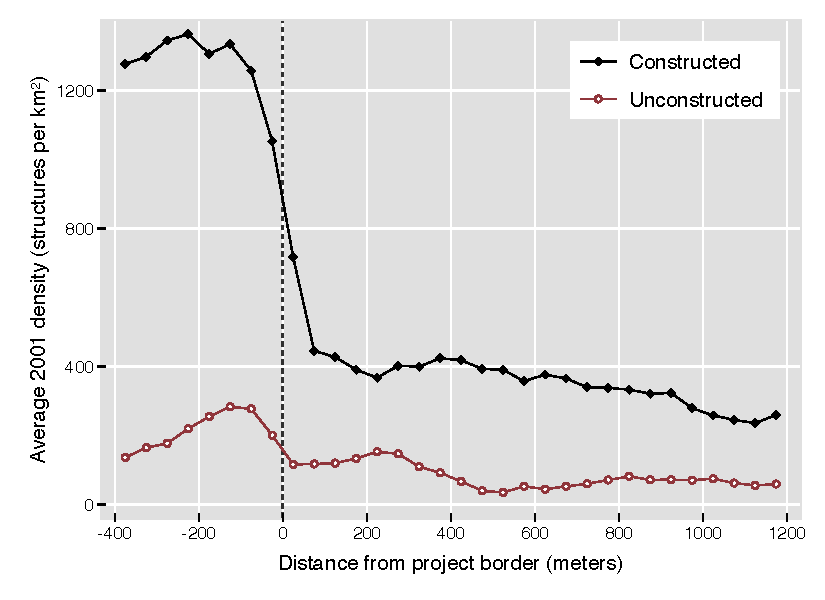
\includegraphics[width=\textwidth,trim={0.3cm .3cm 0.1cm 0cm}, clip=true]{figures/bblu_inf_pre_means_4_4.pdf}
        % \end{subfigure}
        % \vspace{-6mm}
    \end{figure*} 





\begin{table}[h!] 
\caption{Effect of Housing Projects on Socio-demographics}
\label{table:sorting}
\small
\centering
%\caption{Census Composition Estimates }
\vspace{-2mm}
\begin{tabular}{lDDDDD}
\toprule
& \small (1) & \small (2) & \small (3) & \small (4)& \small (5)\\
& \small Age & \small P.O.B. not Gauteng & \small Unemployed & \small Years of Education & \small Monthly Income \\ \midrule 
\textbf{Greenfield} \\   inside project      &      -1.409\textsuperscript{c}&      -0.048                   &       0.140\textsuperscript{a}&      -1.165\textsuperscript{b}&   -1486.342\textsuperscript{c}\\
                    &     (0.749)                   &     (0.052)                   &     (0.051)                   &     (0.451)                   &   (855.477)                   \\[0.01em]
0-300m outside project &      -0.906                   &      -0.100\textsuperscript{b}&       0.139\textsuperscript{a}&      -0.774\textsuperscript{b}&   -1189.553                   \\
                    &     (0.718)                   &     (0.044)                   &     (0.047)                   &     (0.365)                   &  (1030.247)                   \\[0.01em]
300-600m outside project&      -0.874                   &      -0.058                   &       0.043                   &      -0.134                   &    -974.465                   \\
                    &     (0.905)                   &     (0.046)                   &     (0.057)                   &     (0.344)                   &  (1156.804)                   \\[0.8em] 
\textbf{In-Situ Upgrading} \\   inside project      &       0.434                   &      -0.119\textsuperscript{c}&       0.017                   &       0.321                   &    1488.620                   \\
                    &     (0.907)                   &     (0.065)                   &     (0.035)                   &     (0.250)                   &  (1572.224)                   \\[0.01em]
0-300m outside project &      -0.246                   &      -0.036                   &       0.025                   &       0.442                   &    1706.076                   \\
                    &     (0.870)                   &     (0.058)                   &     (0.042)                   &     (0.277)                   &  (1579.078)                   \\[0.01em]
300-600m outside project &      -0.775                   &      -0.004                   &       0.034                   &      -0.007                   &    -593.232                   \\
                    &     (0.920)                   &     (0.052)                   &     (0.037)                   &     (0.271)                   &  (1370.201)                   \\[0.8em]
\textbf{Other} \\   inside project      &       0.564                   &       0.014                   &      -0.013                   &       0.585\textsuperscript{a}&    2971.996\textsuperscript{a}\\
                    &     (0.557)                   &     (0.041)                   &     (0.032)                   &     (0.209)                   &   (960.085)                   \\[0.01em]
0-300m outside project &       1.158\textsuperscript{c}&       0.069\textsuperscript{c}&      -0.015                   &       0.163                   &    1048.665                   \\
                    &     (0.597)                   &     (0.037)                   &     (0.029)                   &     (0.161)                   &   (831.451)                   \\[0.01em]
300-600m outside project &       0.593                   &       0.023                   &      -0.001                   &       0.093                   &    1389.669\textsuperscript{c}\\
                    &     (0.556)                   &     (0.034)                   &     (0.028)                   &     (0.169)                   &   (746.539)                   \\[0.8em]
Mean Outcome 2001   &       27.30                   &        0.37                   &        0.47                   &        8.27                   &    2,482.85                   \\
Mean Outcome 2011   &       28.29                   &        0.43                   &        0.33                   &        9.68                   &    4,512.03                   \\
R$^2$               &       0.201                   &       0.154                   &       0.206                   &       0.395                   &       0.185                   \\
\# projects         &         314                   &         314                   &         314                   &         314                   &         314                   \\
N project areas     &       3,656                   &       3,655                   &       3,655                   &       3,655                   &       3,654                   \\
N spillover areas   &       4,201                   &       4,197                   &       4,196                   &       4,197                   &       4,195                   \\
N                   &      12,733                   &      12,726                   &      12,725                   &      12,726                   &      12,722                   \\

\bottomrule
\multicolumn{6}{l}{\footnotesize Standard errors clustered at the project level in parenthesis. \textsuperscript{c} p$<$0.10, \textsuperscript{b} p$<$0.05, \textsuperscript{a} p$<$0.01  }\\
\multicolumn{6}{l}{\footnotesize P.O.B. means ``place of birth.''  Monthly income is in Rands.}
\end{tabular}
\end{table}




\end{document}


